\documentclass{sig-alternative}
% \documentclass[conference]{IEEEtran}
\usepackage{color}
\usepackage{listings}
\usepackage{graphicx} 
\usepackage{multirow}
\usepackage[table,xcdraw]{xcolor}
\usepackage{cite}
\usepackage{paralist}
\usepackage[table,xcdraw]{xcolor}
\usepackage{siunitx}
\usepackage{rotating}
\usepackage{eqparbox}


\usepackage[framemethod=tikz]{mdframed}
\usepackage{lipsum}
\usetikzlibrary{shadows}
\newmdenv[tikzsetting= {fill=white!20},roundcorner=10pt, shadow=true]{myshadowbox}




\usepackage{graphics}
\usepackage{colortbl} 
\usepackage{multirow}
\usepackage{mathptmx} \usepackage[scaled=.90]{helvet} \usepackage{courier}
\usepackage{balance}
\usepackage{picture}
% \usepackage{multirow}
\usepackage[table,xcdraw]{xcolor}
\usepackage{soul}

\usepackage{fourier} 
\usepackage{array}
\usepackage{makecell}

\renewcommand\theadalign{cb}
\renewcommand\theadfont{\bfseries}
\renewcommand\theadgape{\Gape[4pt]}
\renewcommand\cellgape{\Gape[4pt]}

\usepackage{verbatim}
\usepackage{algorithm}
\usepackage{algorithmicx}
\usepackage{algpseudocode}
\usepackage[export]{adjustbox}
\renewcommand{\footnotesize}{\scriptsize}
\definecolor{lightgray}{gray}{0.8}
\definecolor{darkgray}{gray}{0.6}
\renewcommand{\algorithmicrequire}{\textbf{Input:}}
\renewcommand{\algorithmicensure}{\textbf{Output:}}
\usepackage[table]{xcolor}
\definecolor{Gray}{rgb}{0.88,1,1}
\definecolor{Gray}{gray}{0.85}
\definecolor{Blue}{RGB}{0,29,193}
\newcommand{\G}{\cellcolor{green}}
\newcommand{\Y}{\cellcolor{yellow}}


\definecolor{MyDarkBlue}{rgb}{0,0.08,0.45} 
\lstset{
    language=Python,
    basicstyle=\ttfamily\fontsize{2.7mm}{0.8em}\selectfont,
    breaklines=true,
    prebreak=\raisebox{0ex}[0ex][0ex]{\ensuremath{\hookleftarrow}},
    frame=l,
    showtabs=false,
    showspaces=false,
    showstringspaces=false,
    keywordstyle=\bfseries,
    emph={furthest,gale,better,improved,where,fastmap,split,project,mutate,mutate1}, emphstyle=\bfseries\color{blue},
    stringstyle=\color{green!50!black},
    commentstyle=\color{gray}\itshape,
    numbers=left,
    captionpos=t,
    escapeinside={\%*}{*)}
}


%%% graph
\newcommand{\crule}[3][darkgray]{\textcolor{#1}{\rule{#2}{#3}}}
%\newcommand{\rone}{\crule{1mm}{1.95mm}}
%\newcommand{\rtwo}{\crule{1mm}{1.95mm}\hspace{0.3pt}\crule{1mm}{1.95mm}}
%\newcommand{\rthree}{\crule{1mm}{1.95mm}\hspace{0.3pt}\crule{1mm}{1.95mm}\hspace{0.3pt}\crule{1mm}{1.95mm}}
%\newcommand{\rfour}{\crule{1mm}{1.95mm}\hspace{0.3pt}\crule{1mm}{1.95mm}\hspace{0.3pt}\crule{1mm}{1.95mm}\hspace{0.3pt}\crule{1mm}{1.95mm}} 
%\newcommand{\rfive}{\crule{1mm}{1.95mm}\hspace{0.3pt}\crule{1mm}{1.95mm}\hspace{0.3pt}\crule{1mm}{1.95mm}\hspace{0.3pt}\crule{1mm}{1.95mm}}
\newcommand{\quart}[3]{\begin{picture}(100,6)%1
{\color{black}\put(#3,3){\circle*{4}}\put(#1,3){\line(1,0){#2}}}\end{picture}}
\definecolor{Gray}{gray}{0.95}
\definecolor{LightGray}{gray}{0.975}
% \newcommand{\rone}{}
% \newcommand{\rtwo}{}
% \newcommand{\rthree}{}
% \newcommand{\rfour}{} 
% \newcommand{\rfive}{}
\newcommand{\wei}[1]{\textcolor{red}{Wei: #1}} 
\newcommand{\Menzies}[1]{\textcolor{red}{Dr.Menzies: #1}} 
%% timm tricks
\newcommand{\bi}{\begin{itemize}}%[leftmargin=0.4cm]}
\newcommand{\ei}{\end{itemize}}
\newcommand{\be}{\begin{enumerate}}
\newcommand{\ee}{\end{enumerate}}
\newcommand{\tion}[1]{\S\ref{sect:#1}}
\newcommand{\fig}[1]{Figure~\ref{fig:#1}}
\newcommand{\tab}[1]{Table ~\ref{tab:#1}}
\newcommand{\eq}[1]{Equation~\ref{eq:#1}}
\newcommand{\what}{{\bf WHAT }}

%% space saving measures

%\usepackage[shortlabels]{enumitem}  
\usepackage{url}
% \def\baselinestretch{1}


% \setlist{nosep}
%  \usepackage[font={small}]{caption, subfig}
% \setlength{\abovecaptionskip}{1ex}
%  \setlength{\belowcaptionskip}{1ex}

%  \setlength{\floatsep}{1ex}
%  \setlength{\textfloatsep}{1ex}
%  \newcommand{\subparagraph}{}

% \usepackage[compact,small]{titlesec}
% \DeclareMathSizes{7}{7}{7}{7} 
% \setlength{\columnsep}{7mm}


% \usepackage[svgnames]{xcolor}
% \usepackage[framed]{ntheorem}
% \usepackage{framed}
% \usepackage{tikz}
% \usetikzlibrary{shadows}
% %\newtheorem{Lesson}{Lesson}
% \theoremclass{Lesson}
% \theoremstyle{break}


 
\begin{document}
% \conferenceinfo{FSE}{'15 Bergamo, Italy}
\title{Faster Discovery  of Faster Programs \\from Software Product Lines} 
\numberofauthors{2}
\author{
        \alignauthor Vivek Nair, Tim Menzies, Xipeng Shen 
        \affaddr{Computer Science, North Carolina State University, Raleigh, USA}
        \email{vivekaxl, tim.menzies, xipengshen@gmail.com}
    \and  
        \alignauthor Norbert Siegmund, Sven Apel \\
        \affaddr{Computer Science, University of Passau, Germany}\\
        \email{norbert.siegmund, apel@uni-passau.de}
       }

\maketitle 
\thispagestyle{plain}
\pagestyle{plain}
\begin{abstract}
Prior work on predicting performance scores for software systems generated from
configurable software systems suffered from either (a)~needing far too many samples
of system variants or (b)~large variances in their predictions.
Both these problems can be avoided using the \what spectral learner. \what, like prior work, utilizes the relationship between the selected features of a system variant to predict the performance score of the variant.  
\what   proposes a novel method, which uses the spectrum (eigenvalues) of the distance matrix
between configurations of a configurable software system to perform dimensionality reduction. Within that
reduced configuration space, many closely associated configurations can be studied
by executing just a few samples. For example, for the programs studied
here, a few dozen samples yield accurate and stable predictors - less than 10\% prediction error with a standard deviation of less than 3\%.  
Also, when compared to a prior state-of-the-art approach, our method (a)~required  
25\% to 50\% less samples to achieve the same error rates
and (b)~its predictions are four to sixteen times more accurate. 
%unclear: (i.e., much mean errors and standard deviations on the errors, refer to Figure 9-11)

Further, the predictive model generated by
\what along with the sampling techniques can be used by optimizers to discover configurations that closely
approach the optimal performance scores of all possible configurations of a configurable software system.
\end{abstract}

% A category with the (minimum) three required fields
\vspace{1mm}
\noindent
{\bf Categories/Subject Descriptors:} 
D.2 [Software Engineering];
I.2.6 [Artificial Intelligence]: Induction

 
%\vspace{1mm}
\noindent
{\bf Keywords:} Performance Prediction, 
Active Learning, 
Decision Trees,
Search-based Software Engineering, Sampling.
\pagenumbering{arabic} %XXX delete before submission
 
\begin{comment} 
\end{comment}
 
\section{Introduction}
 
%==Are these comments?== 
%Are feature/variability models too abstract for concrete reasoning?
%Or is it possible to use these models to predict specific properties 
%of programs generated from them? 

Feature or variability models are high-level descriptions of the commonalities and variabilities across related software systems. 
They can be used to derive a set of features (i.e., a configuration) to customize the software behavior. 
That is, each feature combination gives rise to a particular variant of the system which has a particular performance measure.

Feature models have received much attention in literature.
For example, in 1990 Kang et al. published their article on feature models which describe one notation for product lines. 
It has over 4600 citations~\cite{kang1990feature} and is still the basis for recent work~\cite{lopez15,harman14,sayyad13a,sayyad13b}.
Feature models can also be used to make general conclusions about the quality trade-off between different features, which can be very useful for customizing a configurable software system~\cite{sayyad13a,sayyad13b}. 
But, it is harder to make more specific predictions about, say, the expected software performance scores of system variants. 
Prior work on predicting performance scores from feature models had to compile and execute hundreds to thousands of specific variants~\cite{guo2013variability}. 
Other studies that tried to make far fewer execution samples resulted in predictors that were wildly inaccurate in their performance score predictions.
A more balanced approach by Siegmund et al. in 2012 built predictors for  configurable software systems~\cite{siegmund2012predicting} with had low mean errors however the predictions
 were  unstable with large deviations for prediction accuracy for different configurations (e.g., the standard deviations for the Apache Web server was up to $\sigma = 22.7\,\%$). 
 
%My(Norbert) comment on this: you can't just take the worst heuristic here when the paper was about improving over this worst case...
 %\footnote{The predictions of \cite{siegmund2012predicting} had $\mu=19\%$ errors with $\sigma = 19.5\%$.}
  %that half they time, they could be up to 50\% incorrect\footnote{
 %The range  $\mu \pm 1.5*\sigma$  includes the
 %25th to 75th percentile range of a normal distribution   
%For the \cite{siegmund2012predicting} errors, that range is  0 to 49\%.}. 
% >> Where do you have this data from? Does not match with the paper.
% Vivek: You take the fault rate and standard deviation of the method which uses **almost** same  number of measurements. 
Guo et al.~\cite{guo2013variability} also proposed an incremental method to build a predictor model, which uses incremental random samples with steps equal to number of features of the software system. It suffered from the same problem, as the previous work, of unstable predictions (e.g., predictions had a mean error of up to 22\,\% with a standard deviation of up 46\%). Sarkar et al. ~\cite{sarkar2015cost} proposed a way (using few measurements) to quickly compute  the number of evaluation needed to find a stable predictor. The predictor performed better than \what however large number of measurements made it unfeasible for practical use ( 13\% of the total configuration compared to 3\% used by \what).


This paper presents \what, a {\em spectral learner}     that finds 
accurate and  stable predictions of system variants generated from configurable software systems.
\what explores the spectrum (eigenvalues) of the distance matrix
between  features or configurations to perform dimensionality reduction. The reduced
space is then queried to find a small number of representative examples, which is used to
build a predictive model for performance scores (using a decision tree learner~\cite{breiman1984}). The predictive models developed by using \what, along with the sampling techniques, are compared with models developed by Siegmund et al.~\cite{siegmund2012predicting} and Guo et al.~\cite{guo2013variability}. 
For the feature models tested here (Berkeley DB, Apache Web server, SQLite, LLVM and x264 video encoder),
the  predictions are more accurate and have a substantially lower variance than those of Siegmund et al. and Guo et. al \footnote{The prediction in this paper have $\mu=6\%$ error and $\sigma=2\%$.}.


Importantly, our predictions were found using few samples of total feature/configuration space
(number of samples ranges between 16 to 64 executions).
This is significant and most surprising  since some of the systems explored here have up
to millions of possible variations. This result is useful to the community because data collection in case 
of large feature models can be very expensive.

This is a result with a large industrial utility.
In their recent paper, Xu et al. documented the  difficulties developers face
with understanding  the configuration options (i.e., features) of their systems~\cite{xu2015hey}.
Delivered systems have large numbers of configuration options, and the number of  configuration options tends to grow linearly
with time. Consequently, developers  struggle to understand both the current options as well as all the new options.
As a result, developers tend to ignore over $\frac{5}{6}$ths of the configuration options. 
This poor understanding of the configuration space has an economic cost:  for one system (Hadoop clusters),  Xu et al. reported that ``configuration
issues are the dominant source of support cost''~\cite{xu2015hey}. 
Based on the Xu et al. study, it is clear that developers need better tools for understanding the 
consequences of all the configuration options (e.g., such as \what).


The contributions of this paper are:
\bi
\item A new effective sampling strategy for predicting performance metrics of configurable software systems from feature/variability models. The sampling strategy uses an approximate to the first principal component of the feature space to recursively cluster it and uses only a few points as a representative of each cluster;
\item We implement the approach and demonstrate its practicality and generality by conducting experiments on six real-world configurable software systems (see figure ~\ref{fig:systems}). The results show that our approach is more accurate (lower mean error) and more stable (lower standard deviation) than related approaches;
\item We conduct a comparative analysis with the state-of-the-art techniques and demonstrate how our approach outperform prior techniques. A key finding is the utility of principal component of configuration space to  find informative samples from an otherwise large configuration space.
\ei

The rest of the paper is organized as follows. Section 2 defines the terms used in the paper. Section 3 describes the background of the problem we are trying to tackle along with the data sets used in the experiments. Section 4 further explores the research question and finds association among them. Section 5 describes the experiment setup etc. Section 6 discusses the results and Section 7 the related work. This paper concludes after mentioning the threats to validity.


\begin{figure}[!hb]\small
\begin{tabular}{|p{.95\linewidth}|}\hline
\textbf{Berkeley DB CE} is an embedded database system written in C. It is one of the most deployed databases in the world due to its low binary footprint and its configuration abilities. We used the benchmark provided by the vendor to measure response time.

\textbf{Berkeley DB JE} is a complete re-development in Java with full SQL support. Similarly, we used a benchmark provided by the vendor measuring response time.

\textbf{Apache} is a prominent open-source Web server that comes with various configuration options. To measure performance, we used the tools autobench and httperf to generate load on the Web server. We increased the load until the server could not handle any further requests and marked the maximum load as the performance value.

\textbf{SQLite} is an embedded database system deployed over several millions of devices. It supports a vast number of configuration options in terms of compiler flags. As benchmark, we used the benchmark provided by the vendor and measured the response time.

\textbf{LLVM} is a compiler infrastructure written in C++. It provides configuration options to tailor the compilation process. As benchmark, we measured the time to compile LLVM's test suite.

\textbf{x264} is a video encoder in C that provides configuration options to adjust output quality of encoded video files. As a benchmark, we encoded the Sintel trailer (735\%MB) from avi to the xH.264 codec and measured encoding time.\\\hline
\end{tabular}
\caption{Systems studied in this paper.}\label{fig:systems}
\end{figure}


\section{Definitions}

In this section, we formalize the problem of predicting performance scores of configurable software systems. These systems have a set $X$ of Boolean configurations  also referred to as features or independent variables. If a feature is selected in a configuration, it corresponds to $True$ and $False$ otherwise. We represent the features as a vector F=  $<f_1$,$f_2$, ..., $f_N>$, where $N$ is the number of features of the software systems. Each valid instance of the vector (i.e., a configuration) has a corresponding performance score associated to it. The software systems used to validate our method are described in Figure \ref{fig:systems}.
Note, with ``predicting performance scores'', we 
mean predicting performance measures of the system while executing the test suite provided by the manufacturers. Given below are details about the various performance measure associated to  each system:
\begin{description}
\item[Apache:]  \textbf{Request rates} at which the web server stops responding. 
\item[BDBC, BDBJ, SQLite:] The \textbf{time} required to execute the vendor specific benchmark. 
\item[LLVM:] The \textbf{time} LLVM needs to compile its standard test suite. 
\item[x264:] \textbf{Time}   to encode the video trailer Sintel (735 MB). 
\end{description}

These definitions tie our results to particular test suites.
If that test suite was to change, then a  new
performance scores study would need  to be conducted. Ideally, such new predictors
can be quickly built using very few additional samples-- in which case, the methods
of this paper would be most relevant.

 
\begin{figure}[!tb]
\frame{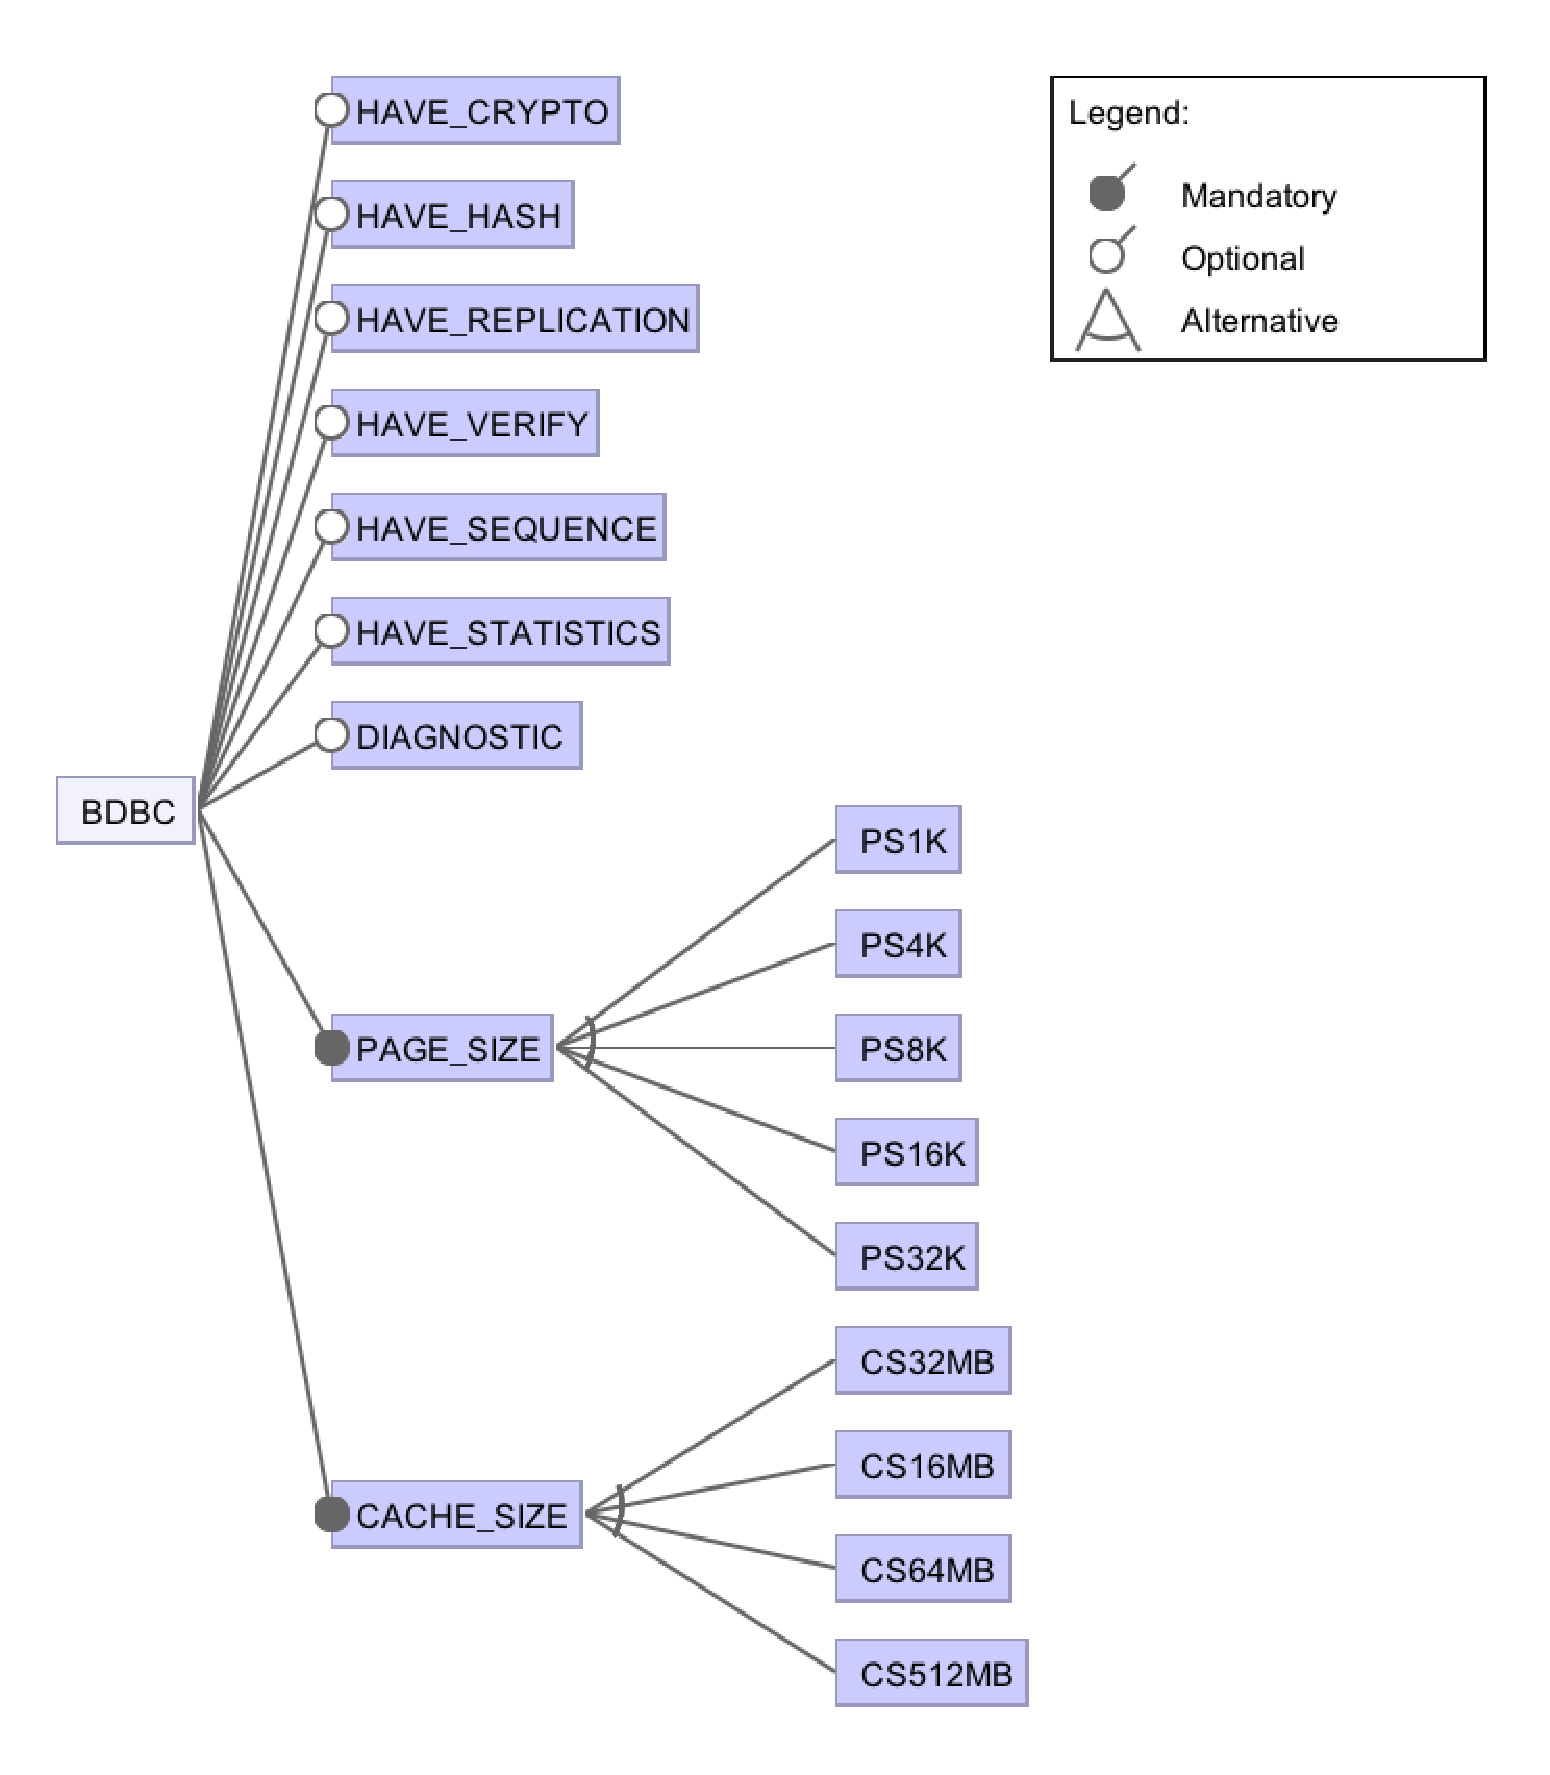
\includegraphics[width=0.95\linewidth]{Figures/BDBC.eps}}
\caption{ Berkeley database feature model   (``C'' version). }\label{fig:bdbc}
\end{figure}
    


\begin{figure}[!tb]
\scriptsize
\begin{tabular}{llllll}
  \hline
Project & Domain & Lang. & LOC & Features & Config\\\hline
Berkeley DB(BDBC)   & Database & C & 219,811 & 18 & 2560\\
Berkeley DB(BDBJ)   & Database & Java & 42,596 & 32  & 400\\
Apache & Web Server & C & 230,277 & 9 & 192\\
SQLite & Database & C & 312,625 & 39 & 3,932,160\\
LLVM & Compiler & C++ & 47,549 & 11 & 1024\\
x264 & Video Enc. & C& 45,743 & 16 & 1152\\\hline
\end{tabular}
\caption{Feature models studied in this paper. For details on these systems,
see \fig{systems}.}
\label{fig:subjectsystems}
\end{figure}




\section{Background}  

\subsection{Feature Models}
We represent a configurable software systems using Kang's feature model (FM) notation, which defines all valid feature combinations. 
As shown in figure~\ref{fig:bdbc}, a feature model can be presented as a tree-like structure that defines relationships among features.   Features are represented as a set of Boolean variables. 

However, Feature models can be far more elaborate than shown in \fig{bdbc}. 
A feature model of the LINUX kernel~\cite{sayyad13b} contains thousands of features and hundreds of thousands of  {\em cross-tree constraints} --- choices in one branch that rule out choices in other branches. 
Without those constraints, it takes linear time to generate possible variants via a simple
top-down descent of the model. With those constraints, variant generation becomes NP-hard and can
 defeat state-of-the-art theorem provers~\cite{pohl11} in particular, for larger feature models.
 
 
 
In practice, not all feature models are as complex as in one of LINUX.
\fig{subjectsystems} details the feature models used in this study. While
they seem to be small with only few dozen features, the last column in that table lists hundreds
to millions of configurations they give generate.


\subsection{Predicting Performance Scores}\label{sect:addit}
The literature offers two approaches: a {\em maximal sampling} and a {\em minimal sampling} methods, to predict the performance scores of products generated from feature or variability models. 

In the {\em maximal sampling} method, we compile all  possible configurations and record the associated performance scores. Maximal sampling  can be impractically slow.
For ex., the performance data used in this paper required  26 days of CPU time to collect (and much longer, if we also count the time required
 for compiling the code prior to execution). 
 Other researchers have commented that,  in 
 real world scenarios, the cost of acquiring optimal configuration is overly expensive and time consuming \cite{weiss2008maximizing}.
 
 If collecting performance scores on all configurations is impractical,  {\em minimal sampling } 
 is used to intelligently select and execute   just enough configurations (i.e., samples) to build
 predictive models.
 Zhang et al.~\cite{zhang2015performance} approximate the
 systems as a Fourier series, after which they can derive an expression showing how many configurations must be studied
 to build predictive models with error $\epsilon$. While a theoretically satisfying result, that approach still needs thousands to hundreds of thousands of executions of sample
 configurations.  

Another set of approaches are the four "additive" {\em minimal sampling} methods for Siegmund et al.~\cite{siegmund2012predicting}.
Their first method, called feature-wise ({\em FW}), is their basic method and 
three of these methods are    elaborations of their basic method.
To explain FW, we note that from a configurable software system, it is theoretically possible to enumerate many or all of the legal configurations\footnote{Though, in practice, this can be very difficult. For example, in models like the Linux Kernel such an enumeration is practically impossible ~\cite{sayyad13b}.}. 
Each such
configuration is a vector of $n$ booleans where $n_i$ indicates if this configuration uses feature $f_i$.
Using this information it  is possible to isolate examples of how much each feature individually contributes to the total runtime:
\be
\item Find a pair of  configurations $C_1,C_2$  where $C_2$ uses exactly the same features as $C_1$, plus just one  extra feature $f$.
\item Set the runtime $\Pi(f)$ for feature $f$ to be the difference in the performance scores between $C_2$ and $C_1$.
\item The runtime  for a new configuration  $C_i=\{f_1,f_2,f_3, ...\}$, that has not been sampled before,  is the sum of the runtime of its features; i.e.
\begin{equation}
  \Pi(C_i) = \sum_{f_j \in C_i}\Pi(f_j)  
\end{equation}
\ee

Further to the first point, when many pairs such as ${C_1,C_2}$ satisfy the criteria of point~1, Siegmund et al. used the 
pair that mentions the {\em smallest} number of features. Their basic {\em FW} minimal sampling method 
just compiles and executes just these smallest $C_1,C_2$ configurations. 

Siegmund et al. also offered three extensions to the basic method. All these extensions are based on sampling
not just the smallest $C_1,C_2$  pairs but also any configurations with {\em interactions}. 
All the following minimal sampling policies compile and   execute legal configurations selected via one of three heuristics:
\bi
\item[{\em PW (pair-wise):}] For each pair of features, try to find a configuration that contains the pair and has a minimal number of features selected. 
\item[{\em HO (higher-order):}] Select extra configurations, in which three features $a,b,c$ are selected if two of the following know pair-wise interactions exist $(a,b)$ and $(b,c)$ and $(a,c)$.
\item[{\em HS (hot-spot features):}] Select extra configurations that contain features that are
frequently interacting with other features. 
\ei



Guo et al.~\cite{guo2013variability} proposed progressively random sampling methodology which samples in steps of the number of features in the software system. The sampled configuration was used to train a regression tree and which is then used to predict the performance scores of the system. The termination criteria of this technique is based on the heuristic called as $PW$ same as the one proposed by Siegmund et al. 

Sarkar et al. ~\cite{sarkar2015cost} proposed a cost model, which was be used to predict the effort (or cost) required to generate a accurate model. The user can use this score to decide whether to go ahead and build the model. The method proposed by Sarkar et al. randomly samples configuration and uses a heuristic called feature-frequency as a termination criteria. These samples are then used to train a regression tree and the accuracy of model is measured by using a test set (size of train set is equal to size of the test set). One of the four basis function is selected based on how correlated they are to  accuracy measures. This basis function is used to approximate the accuracy-measure curve. The elbow point of the curve is then used as the optimal sample size. Once the optimal size is known, Sarkar et al. uses the model proposed by Guo et al. to build the model.  


The advantage of these methods are that, unlike  the results in Zhang et al., these  methods require only dozens to hundreds of samples. Also, unlike our approach, these sampling heuristics do not require to enumerate all configurations which is important for highly configurable software systems. 
That said, as shown by the experiments later in this paper, the  methods produce estimates with partially large mean error and partially larger variance than the \what method proposed in this paper. Note: in some cases Sarkar et al. build models with lower mean fault rates however, the large number of measurements are required to build such models. 
 

\subsection{Spectral Learning}\label{sect:spect}

The minimal sampling method explored in this paper is based on a spectral learning algorithm
that  explores the spectrum (eigenvalues) of the distance matrix between  configurations.
In theory, such spectral learners are a better way to handle noisy, redundant, and tightly inter-connected variables, for the following reasons.
When data sets have many irrelevancies or closely associated data parameters $d$, then
only a few $e \ll d$ eigenvectors are required to characterize that data.
In that reduced space:
\bi
\item
Multiple inter-connected variables $i,j,k \subseteq d$ can be represented
by a single eigenvector.
\item
Noisy variables from $d$ are
ignored, because they  do not contribute to the signal in the data.
\item
Variables  become (approximately) parallel lines
in $e$ space. For  redundancies \mbox{$i,j \in d$}, we
can ignore $j$
since effects that change over $j$ also
change in the same way over $i$.
\ei
That is, in theory, samples of configurations drawn via an eigenspace sampling method
would not get confused by noisy, redundant, or tightly inter-connected variables. Accordingly,
we expect predictions built from that sample to have  lower mean errors and lower variances on that error.

Spectral methods have been used before for a variety of data mining applications~\cite{kamvar2003spectral}.
Algorithms, such as PDDP~\cite{boley98} use spectral methods, such as principle component analysis (PCA) to
recursively divide data into smaller regions.  Software analytics researchers use spectral methods (again, PCA) as a pre-processor prior to data mining  to reduce noise in software-related data sets~\cite{Theisen15}.
However, to the best of our knowledge, spectral methods have not been used before in software engineering as a basis of a minimal sampling policy.



\what is somewhat different from other spectral
learners explored in, for instance, image processing applications~\cite{shi00}.
The image processing papers do not address
defining a minimal sampling policy to predict performance scores.
Also, standard spectral method requires some $O(N^2)$ matrix multiplication to compute the components
of PCA~\cite{ilin10}. Worse, in the case of hierarchical division methods such as PDDP,
that polynomial time inference must be repeated at every level of the hierarchy.
Competitive results can be achieved
using an $O(2N)$ analysis that we have developed previously~\cite{me12d}, which is  based on  a heuristic proposed by Faloutsos and Lin~\cite{Faloutsos1995} (which Platt has shown computes a Nystr\"om approximation to the first component of PCA~\cite{platt05}).
  
Our approach inputs $n$
examples $n_1,n_2,..$. The FASTMAP heuristic
picks any
point $n_i$ at random and  finds
 the point  {\em West}~$\in n$ that is
furthest away from $n_i$.
FASTMAP then finds the point {\em East}~$\in n$
that is furthest from {\em West}.
We say that the line between {\em West} and {\em East} has  length  
$c=\mathit{dist}(\mathit{West},\mathit{East})$ (look at equation 2).
\what uses FASTMAP recursively to divide all the configurations as follows.
We iterate over $n_i \in n$
to find
$a=\mathit{dist}(n_i,\mathit{West})$,
$b=\mathit{dist}(n_i,\mathit{East})$,
$x=(a^2 + c^2 - b^2)/(2c)$.
This  $x$ value is the projection of $n_i$
on the line  running  from {\em East} to {\em West}.  We divide
the examples based on the median value of the projection($x$),
then recurse on each half. The recursion on
$n$ initial
examples stops when a sub-region
contains less that  $M$ examples (e.g. 
$M=\sqrt{|n|}$).
We explore this approach for three reasons:
\bi
\item
{\em It is very fast}:
This process requires only $2*|n|$ distance comparisons
per level of recursion, which is far less than the $O(|n|^2)$
required by PCA~\cite{Du2008}
or other  algorithms such as K-Means~\cite{hamerly2010making}.
\item
{\em It is not domain specific}:
This approach is general unlike traditional PCA. It does not make any assumption that all the variables are numeric. As shown in equation 2, we can approximate distances for both numeric and non-numeric data.

\begin{equation}
    dist(x, y) = 
    \begin{cases}
        \sqrt{\sum_i(x_i-y_i)^2},& \text{if $x_i$ and $y_i$ is numeric}\\
        \begin{cases}
            0, & \text{ if $x_i$ == $y_i$}\\
            1, & \text{ otherwise}\\
        \end{cases}
        ,& \text{if $x_i$ and $y_i$ is boolean}\\
    \end{cases}
\end{equation}

\item
{\em Explore the underlying dimension of the search space (configuration space)}:
This technique explores the underlying dimension (first principal component) without getting confused by noisy, related and highly associated variables (see section 3.3).

\ei

\subsection{Spectral Sampling}\label{sect:sample}
When the above clustering method terminates, our  sampling policy (which we will call $S_1$:Random) is then applied:
\begin{quote}
$S_1$: Random sampling: Compile and execute one  configurations,  picked at random, from each leaf cluster.
\end{quote}
We use this sampling policy, because (as we will show later) $S_1$:Random sampling performs better than:
\bi
\item $S_2$: East-West sampling: compile and execute the {\em East} and {\em West} poles of the leaf clusters;
\item $S_3$: Exemplar sampling: compile and execute all items in all leaves and return the one
with lowest performance score.
\ei
Note that $S_3$ is {\em not} a {\em minimal} sampling policy (since it executes all configurations). 
We use it here as one  baseline
against which we can compare the other, more minimal, sampling policies. In the results
that follow, we also compare our 
sampling methods against another baseline using information gathered after executing
all configurations.

\subsection{Regression Tree Learning}
After collecting the data using one of the sampling policies, we then use  CART regression tree learner \cite{breiman1984} to build a predictor for performance scores. Regression tree learners seek the attribute range split that most increases
our ability to make accurate predictions.
CART explores splits which divide $n$ samples  into  $n_1$ and $n_2$ samples, where each sample  has a  standard deviation on the target variable of $\sigma_1$ and  $\sigma_2$.
CART finds the ``best'' split is defined as the split which minimizes $\frac{n_1}{n}\sigma_1 + \frac{n_2}{n}\sigma_2$.
Using this best split, CART divides the data recursively.
 

The validity of the predictors built by CART  is then tested on testing data. There is no intersection between the training data (spectral learning processing) and the testing data (see below for details). 
For each  test item, we find out how long it {\em actually} takes to run the corresponding variant and compare the actual measured performance to the {\em prediction} from CART. The resulting prediction error is then computed using:
\begin{equation}\label{eq:err}
\mathit{error}=\frac{\mathit{abs}(\mathit{predicted} - \mathit{actual})}{\mathit{actual}}*100
\end{equation}

\section{Research Questions} 
In summary, \what  combines:
(1) the FASTMAP method of Faloutsos and Lin~\cite{Faloutsos1995};
(2)~a spectral learning algorithm initially   inspired by    Boley's PDDP system~\cite{boley98}, which we modify
by replacing  PCA with FASTMAP (called
``WHERE'' in prior work ~\cite{me12d});
(3)~the $S_1$:Random sample method that explores the leaf clusters found by this recursive division;
and (4)~the CART regression tree learner that converts the data from the samples collected by $S_1$:Random
into a runtime prediction model~\cite{breiman1984}.
That is,
\begin{center}
\begin{tabular}{rcl}
WHERE& = &PDDP - PCA + FASTMAP\\ 
\what& =  & WHERE + $S_1$:Random + CART
\end{tabular}
\end{center}
This unique combination of methods has not been previously explored in the
software-engineering literature but is promising because it explores the underlying dimension of the space without getting confused by noisy, redundant, and highly associated variables (see section 3.3).

%Could be removed if space is needed
Since our model explores the spectral space, it might be true that only a small
number of samples are required to explore the whole space.
However, a model built from a very small sample of the available data might
be very inaccurate and unstable i.e. it may exhibit very large mean errors and standard deviations on the error.

%Could be removed if space is needed
Also, if we learn models from small regions of the training data,
then it is  possible that that learner will miss {\em trends} in the data
between the sample points. Such trends are useful when building {\em optimizers};
i.e. devices that input one configuration and propose an alternate
configuration that has, for instance, faster performance scores. Such optimizers might
need to evaluate hundreds to millions of alternate configurations. 
To speed up that process, optimizers can use a {\em surrogate model}\footnote{Also known as response surface methods, meta models, or emulators.}
that  mimics the outputs of a system of interest, while being computationally cheap(er) to evaluate~\cite{loshchilov13}. For example, when optimizing
performance scores, we might ask the CART  for a performance
prediction (rather than compile and execute
configurations).  Note that such surrogate-based
reasoning critically depends on how well the surrogate can guide optimization.


Therefore, to assess our sampling policies, we must consider:
\begin{compactitem}
\item Performance scores generated from our minimal sampling policy;
\item The variance of the error rates when comparing predicted performance score with actual ones;
%the next point should always be true. otherwise, what would be the reason to do that?!
\item The optimization support offered by the performance predictor (i.e., can the model work in tandem with other off-the-shelf optimizers to generate useful solutions).
\end{compactitem}
The above concerns leads to four research questions:
\begin{compactitem}
\item {\bf RQ1:} {\em Can  \what  + $S_1$:Random spectral learning generate good predictions after
executing only a small number of configurations?}
\end{compactitem}
Here, by ``good'' we mean that the predictions found via sampling with \what + $S_1$:Random are as good, or better,
as those generated from more samples.
\bi
\item {\bf RQ2:} {\em
Does less data used in building the models lead to large variance in the predicted values?}
\item {\bf RQ3:} {\em
Can ``good'' surrogate models (to be used in optimizers)
be built from minimal samples?}
\ei
Note that {\bf RQ2, RQ3} are of particular concern with our approach,
since our goal is to sample as little as possible from the configuration space.
\bi
\item {\bf RQ4:} {\em Compared to the state-of-the-art in minimal sampling for
learning performance-score predictors from configurable software systems, how good is \what with $S_1$:Random?}
\ei
To answer this last question, we will compare \what with $S_1$:Random
          against approaches presented in ~\cite{siegmund2012predicting}, \cite{guo2013variability}, \cite{sarkar2015cost}.
 
\section{Experiments}

%\subsection{Reproduction Package}

All the materials required to reproduce this work are available at \url{https://goo.gl/689Dve}.

\subsection{Case Study Materials}

This study explores feature models, along with the performance score measurements obtained from real time measurements, of the configurable software systems listed in \fig{subjectsystems}.
Also, to compare our results from minimal sub-sampling to those obtained 
from a larger sample, we use data sets showing the performance scores associated with
compiling and executing {\em nearly all} configurations\footnote{http://openscience.us/repo/performance-predict/cpm.html}.

We say {\em nearly all} configurations, for the following reasoning. For 
$\frac{5}{6}$ths of our case studies, the number of possible configurations
was not large (192 to 2560). However, the SQLite product line has 3,932,160 
possible configurations-- which is an impractically large number of configurations to explore. Hence, for SQLite, we use the 4500 samples that could
be collected in one day of CPU time (and, in the results shown below,
we will pay particular attention to the variance of the SQLite results).

\subsection{Experimental Rig}


{\bf RQ1} and {\bf RQ2} require the construction and assessment of numerous runtime predictors from small samples
of the data. The following rig implements that construction process.

For each configurable software system, we built a table of data, one row per valid configuration. We then run all configurations of all software systems
and record the performance scores (i.e., that are invoked by a benchmark).
The exception is SQLite in which we measure only the
configurations needed to detect interactions and additionally
100 random configurations to evaluate the accuracy of
predictions.  
To this table, we added a column showing the performance score obtained from the actual measurements for each configuration (refer to section 2).

Next, 20 times, we repeated the following procedure (the figure of 20 repeats was
selected using the central limit theorem). Note that the following rig ensures that
we \textbf{never} test any prediction model on the data used to learn that model.
\bi
\item For each system in \{BDBC, BDBJ, Apache, SQLite, LLVM, x264\},
\bi
\item Randomize the order of the rows in their table of data;
\item For $X$ in \{10, 20, 30, ... , 90\};
\bi
\item Let {\em Train} be the first $X$\,\% of the data 
\item Let {\em Test} be the rest of the data;
\item Pass {\em Train} to \what to find a sample of configurations;
\item Determine the performance scores associated with those configurations (in our rig, this corresponds to a table lookup, but would entail compiling and executing the software variant in a practical setting).
\item Using the {\em Train}  data and their performance scores, build a performance predictor using CART.
\item Using {\em Test}, assess the accuracy of the predictor using the error 
measure of \eq{err}.
\ei
\ei
\ei
{\bf RQ2} requires testing the standard deviation of the predictions. To support that test, we:
\bi
\item Determine the $X$-th point in the above experiments where all predictions stop improving (elbow point);
\item Measure the standard deviation of the error at that point, across our 20 repeats.
\ei
As shown in figure \ref{fig:sampling_accuracy}, all our results plateaued after studying $X=40$\,\% of the valid configurations
 \footnote{Just to clarify one frequently asked question about this work, we note
that our rig ``studies'' 40\,\% of the data. We do not mean that our predictive models
 require accessing the performance scores from the 40\,\% of the data. Rather, by ``study'' we mean   reflect 
 on a sample of configurations to determine what minimal subset of that
sample deserves to be compiled and executed.}.
 Hence to answer {\bf RQ2}, we will compare all 20 predictions at $X=40$\,\%.
 
{\bf RQ3} requires using the regression tree learned in this way as a {\em surrogate model} within an optimization process. To study this research question, we:
\bi
\item Take   $X=40\,\%$ of the configurations;
\item Apply \what with $S_1$:Random to build a CART model using some minimal sample taken from that 40\,\%;
\item Used that CART model within some standard optimizers while searching for 
configurations with least runtime;
\item  Compare the faster configurations found in this manner with the fastest configuration
known for that system.
\ei
This last item requires access to some ``ground truth'' of performance scores for a very
large number of configurations. For this experiment, we have access to that ground truth
(since we have access to nearly all the configurations). While that ground truth is required for this
validation study, we note that, once our methods satisfy this validation study,
they would not not be needed if practitioners choose to use \what in their own work.

As to the optimizers used in this second experiment, for the sake of completeness, we explored
a range of optimizers seen in the   literature:  DE~\cite{storn1997differential}, NSGA-II~\cite{deb00afast}
and our own GALE~\cite{krall2014gale,zuluaga2013active} system.   Normally,
it would be  reasonable to ask
why we used those three, and not the hundreds of other 
optimizers described in the literature~\cite{fletcher13,harman12}. However,
as shown below, all these optimizers in this
domain exhibited  very similar
behavior (all found configurations close to the
best case performance). Hence, the specific
choice of optimizer is not a critical
variable in  our analysis.


\section{Results}


\begin{figure}[!t]
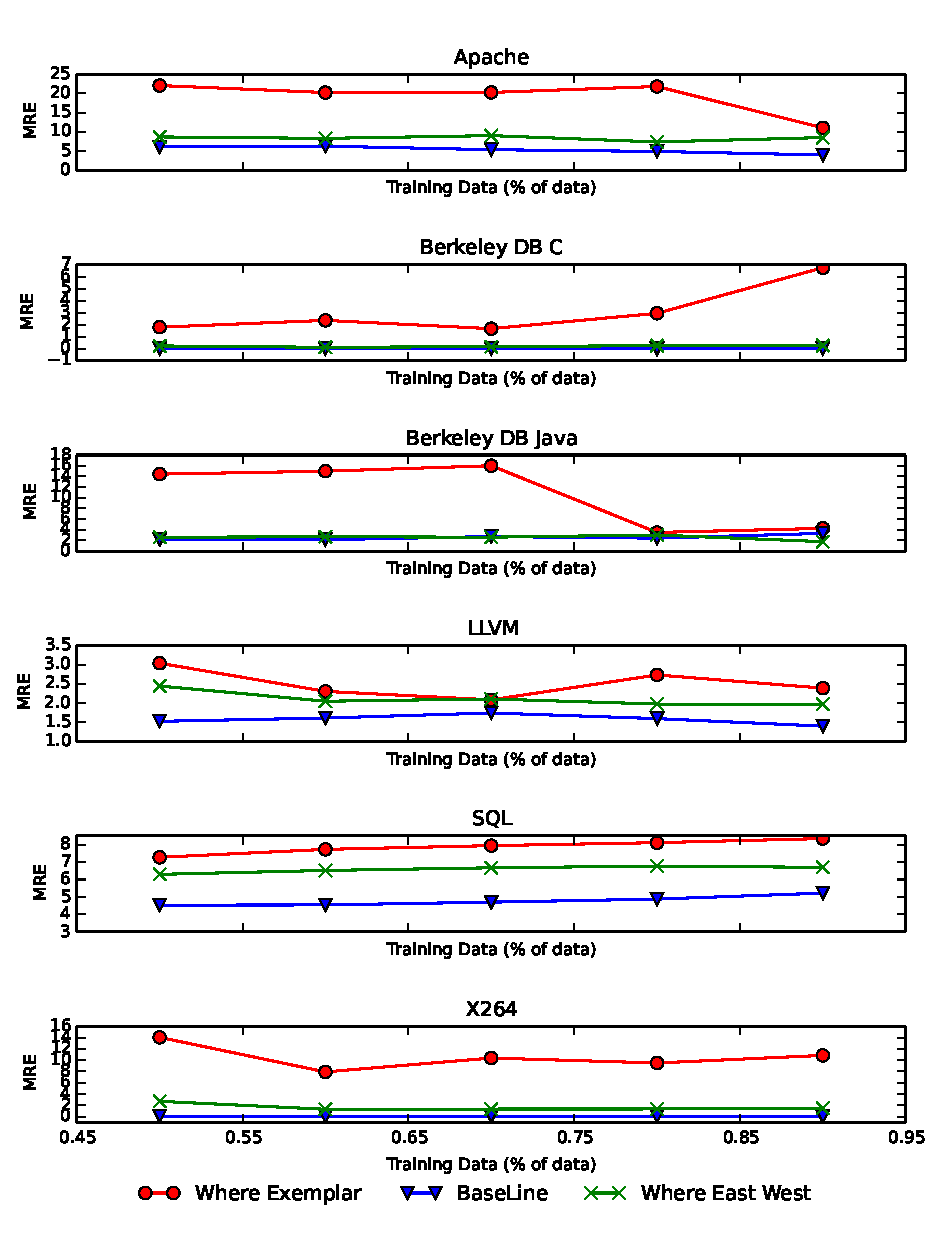
\includegraphics[width=0.9\linewidth]{Figures/SamplingAccuracy.eps}
\caption{Error seen in the predictions made by \what with four different
sampling policies. Note that. on the y-axis,  {\em lower} errors are {\em better}.}
\label{fig:sampling_accuracy}
\end{figure}

\subsection{RQ1}
{\em Can  \what  + $S_1$:Random spectral learning generate good predictions after
executing only a small number of configurations?}

\fig{sampling_accuracy} shows the mean errors of the predictors learned
after taking $X$\,\% of the configurations, then asking  \what and some sampling method
to (a)~find what configurations to measure; then (b)~asking CART to build a predictor
using that execution information. The horizontal axis of those plots shows what $X$\,\%
of the configurations are studied and the vertical axis shows the mean relative error (from \eq{err}).
In that figure:
\begin{compactitem}
\item
The \textcolor{blue}{{\bf blue}} lines on \fig{sampling_accuracy} show a {\em baseline} result
where data from the performance scores of 100\,\% of  configurations were used by CART
to build a runtime predictor.
\item
The other lines show the results using the sampling methods defined in \tion{sample}.
Note that these sampling methods used  runtime data only from a
subset of 100\,\% of the performance scores seen in configurations
from 0 to X\,\%.
\end{compactitem}


The {\em lower} y-axis values  in  \fig{sampling_accuracy} are {\em better} since this shows lower
prediction errors. We found that:
\begin{compactitem}

\item Some software systems exhibit large variances in their error rate, below $X=40$\,\% (e.g., BDBC and BDBJ).
\item Above $X=40$\,\%, there is little effect on other overall change of the sampling methods.
\item
In most of the experiments, the {\em exempler} sampling method $S_3$ shows the highest overall error 
so that it cannot be recommended.
\item Always, the   blue baseline shows the lowest errors, which is to be
expected since predictors built on the baseline have access to all data.
\item
We see a trend that the error of  $S_1$:Random and $S_2$:EastWest are within $5$\,\% of the {\em baseline} results.
Hence, we can recommend these two minimal sampling methods.
\end{compactitem}

\fig{Evaluations} comments on one which  of    $S_1$:Random or $S_2$:EastWest we should recommend.
This figure displays data taken from the $X=40$\,\% point of \fig{sampling_accuracy} and displays
how many performance scores of configurations are needed by our sub-sampling methods (while
reflecting on the configurations seen in the range $0\le X \le 40$. Note that:
\begin{compactitem}
\item
The {\em Exemplar} sampling policy needs up to thousands of performance-score points, 
so it cannot be recommended as minimal sampling policy;
\item The {\em East-West} sampling policy needs twice as much performance-score information as 
the $S_1$:Random {\em random} policy (since $S_2$ uses {\em two} samples per leaf cluster  while
$S_1$:Random uses only {\em one}).
\item $S_1$:Random needs performance-score information on only a few dozen (or less) configurations to generate
the predictions with the lower errors seen in \fig{sampling_accuracy}.
\end{compactitem}
Combining \fig{sampling_accuracy} and \fig{Evaluations} results, we conclude that:

\begin{myshadowbox}
$S_1$:Random is our preferred spectral sampling method and
the answer to {\bf RQ1} is ``yes'', because applying \what + $S_1$: Random, we can (a)~generate runtime predictors
using just a few dozens examples of performance scores; and (b)~those predictions have error rates
within 5\,\% of the error rates seen if predictors built from information about all performance scores.
\end{myshadowbox}

\begin{figure}[!t]
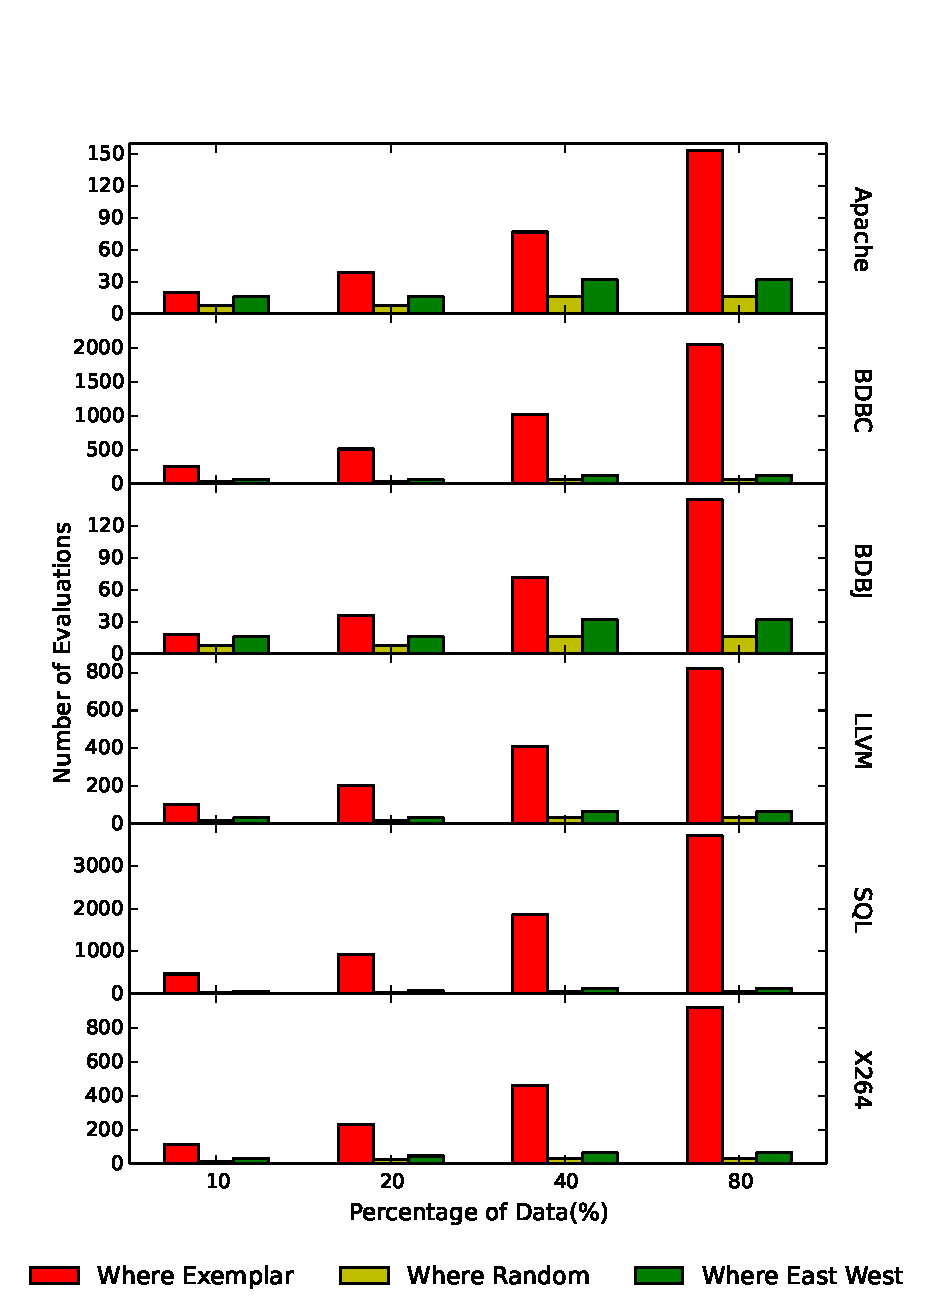
\includegraphics[width=0.9\linewidth]{Figures/evaluation_graph.eps}
\caption{ Comparing evaluations of different sampling policies. We see that the number of configurations evaluated for $S_2$:EastWest is twice as much as $S_1$:Random, since it selects 2 points from each cluster where as  $S_1$:Random selects only one }\label{fig:Evaluations}
\end{figure}


\subsection{RQ2}

{\em
Does less data used in building the models lead to large variance in the predicted values?}\\

Two competing effects can lead to increased or decreased  variance  in 
runtime predictions.
The   less we sample the configuration space,
the less we constrain model generation in that space. Hence, one effect that might be expected
is that models learned
from too few samples can exhibit large variance. 
On the other hand,
a  compensating effect can be introduced by sampling from spectral space
since that space contains fewer confusing variables than that raw data.

\fig{Variance} reports which one of these two competing effects are dominant. 
The \fig{sampling_accuracy} shows that after some initial fluctuations,
after seeing $X=40$\,\% of the data, the variability in predictions reduces to nearly zero.


\begin{figure}[!t]
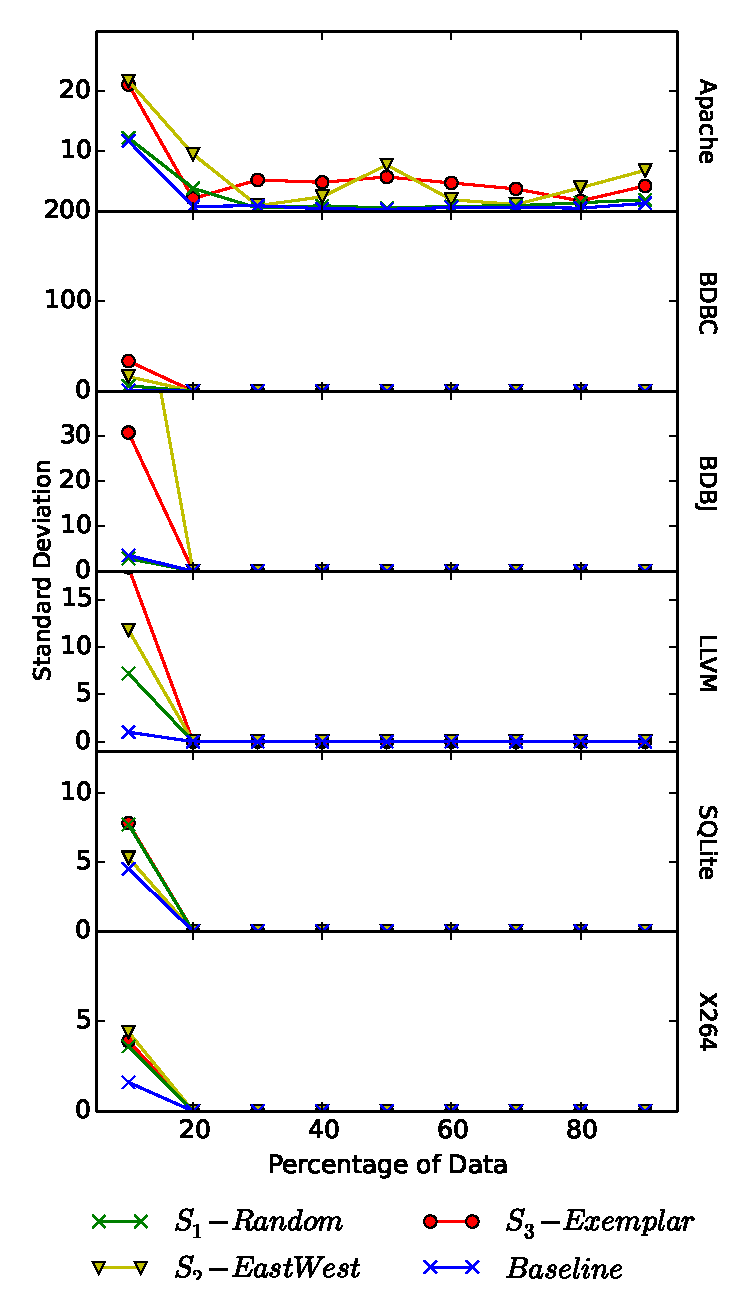
\includegraphics[width=0.9\linewidth]{Figures/Variance.eps}
\caption{Standard deviations seen at various points of  \fig{sampling_accuracy}.}\label{fig:Variance}
\end{figure}

\begin{myshadowbox}
Hence, we answer {\bf RQ2} with ``no'': selecting a small number of samples does not increase variance (at least to say, not in this domain).
\end{myshadowbox}




\subsection{RQ3}

 {\em
Can ``good'' surrogate models (to be used in optimizers)
be built from minimal samples?}

The answers to {\bf RQ1} and {\bf RQ2} recommend using \what+$S_1$:Random to build runtime predictors from a small sample of the data. {\bf RQ3}
asks if that predictor can be used by an optimizer to infer what {\em other} configurations correspond to system variants with fast performance scores?
To answer this question,  we ran  a random set of 100 
configurations, 20 times, then relate that baseline to three optimizers (GALE~\cite{krall2014gale}, DE~\cite{storn1997differential}, NSGA-II~\cite{deb00afast}) using their
default parameters.
 
When these three optimizers mutated existing configurations to suggest new ones,
those mutations were checked against the feature model. Any mutants that violated the feature-model constraints were rejected
and the survivors were ``evaluated'' by asking the CART surrogate model.
%(the  CART regression tree learned from \what+$S_1$:Random, built using the methods of {\bf RQ1}).
These evaluations either rejected the mutant or used it in generation $i+1$, as the basis for a search for more, possibly
better  mutants.




\fig{performance_graph} shows the configurations found by GALE projected onto the ``ground truth'' of the performance scores of nearly
all configurations. Again note that, while we use that ``ground truth'' for the validation of these results, our optimizers 
used only a small percent of that ground truth data in their search for the fastest configurations (see the \what + $S_1$:Random
results of \fig{Evaluations}).


\begin{figure}[!t]
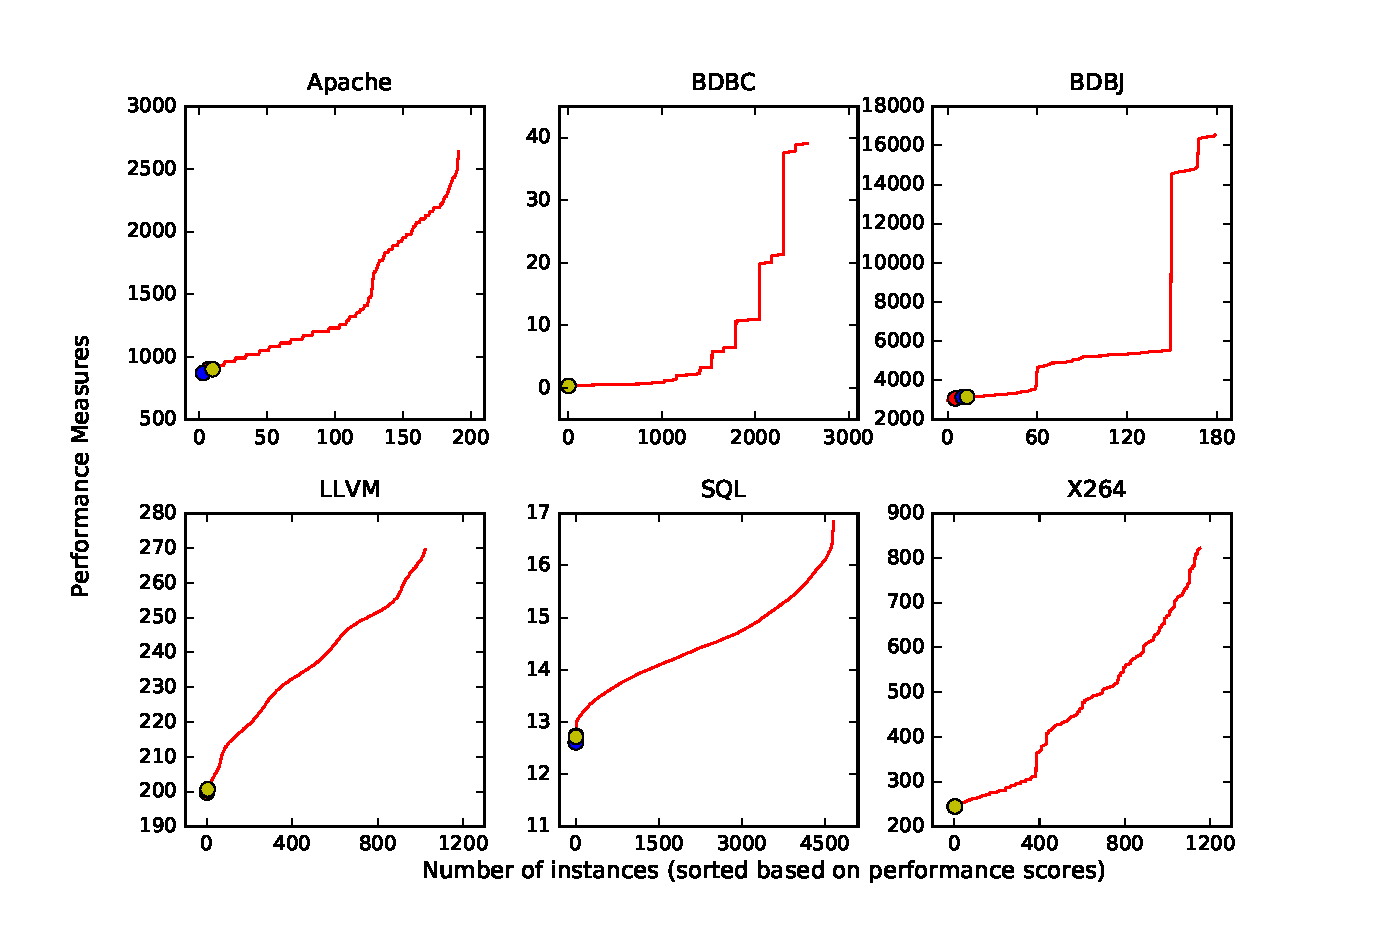
\includegraphics[width=0.9\linewidth]{Figures/optimizer_result.eps}
\caption{Solutions found by GALE (shown as points) laid against the ground truth (all known configuration performance scores) with the exception of SQLite, as this data set does not contain the exhaustive set of configurations and the corresponding performance scores.}\label{fig:performance_graph}
\end{figure}


The important feature of \fig{performance_graph} is that all the optimized configurations fall within 1\,\% of the fastest
configuration in the ground truth (see all the left-hand-side dots on each plot). \fig{external_validity} compares GALE's performance to that of the two other optimizers
used in this study. Note that the performances are nearly identical which leads to the following conclusions:

\begin{myshadowbox}
The answer to {\bf RQ3} is ``yes''--- for optimizing performance scores, we can use surrogates built from few runtime samples. Also, the choice of the optimizer does not critically effect this conclusion.
\end{myshadowbox}


\begin{figure}[h]
\resizebox{3.3 in}{!}{

\begin{tabular}{|l@{~}|l@{~}|l@{~}|l@{~}|l@{~}|l@{~}|l@{~}|l@{~}|l@{~}|l@{~}|l@{~}|l@{~}|l|}
\hline
\multirow{2}{*}{Searcher} & \multicolumn{2}{l|}{Apache} & \multicolumn{2}{l|}{\begin{tabular}[c]{@{}l@{}}Berkeley \\ DB C\end{tabular}} & \multicolumn{2}{l|}{\begin{tabular}[c]{@{}l@{}}Berkeley \\ DB Java\end{tabular}} & \multicolumn{2}{l|}{LLVM} & \multicolumn{2}{l|}{SQLite} & \multicolumn{2}{l|}{X264} \\ \cline{2-13} 
                          & $\mu$         & IQR        & $\mu$                                 & IQR                                  & $\mu$                                   & IQR                                   & $\mu$       & IQR        & $\mu$      & IQR        & $\mu$       & IQR        \\ \hline
GALE                      & 870            & 0          & 0.363                                 & 0.004                                & 3139                                     & 70                                    & 202       & 3.98       & 13.1     & 0.2411     & 248      & 3.3       \\ \hline
DE                        & 840            & 0          & 0.359                                 & 0.002                                & 3139                                     & 70                                    & 200       & 0          & 13.1      & 0          & 244       & 0.003      \\ \hline
NSGA2                     & 840            & 0          & 0.354                                 & 0.005                                & 3139                                     & 70                                    & 200       & 0          & 13.1      & 0.406      & 244       & 0.05       \\ \hline
\end{tabular}}
\caption{The minimum performance scores as found by learners GALE, NSGA-II and DE, for  20 repeated
runs. Mean values are denoted $\mu$ and IQR denotes the 75th-25th percentile.}
\label{fig:external_validity}
\end{figure}



 
\subsection{RQ4}

\begin{figure*}[htbp]
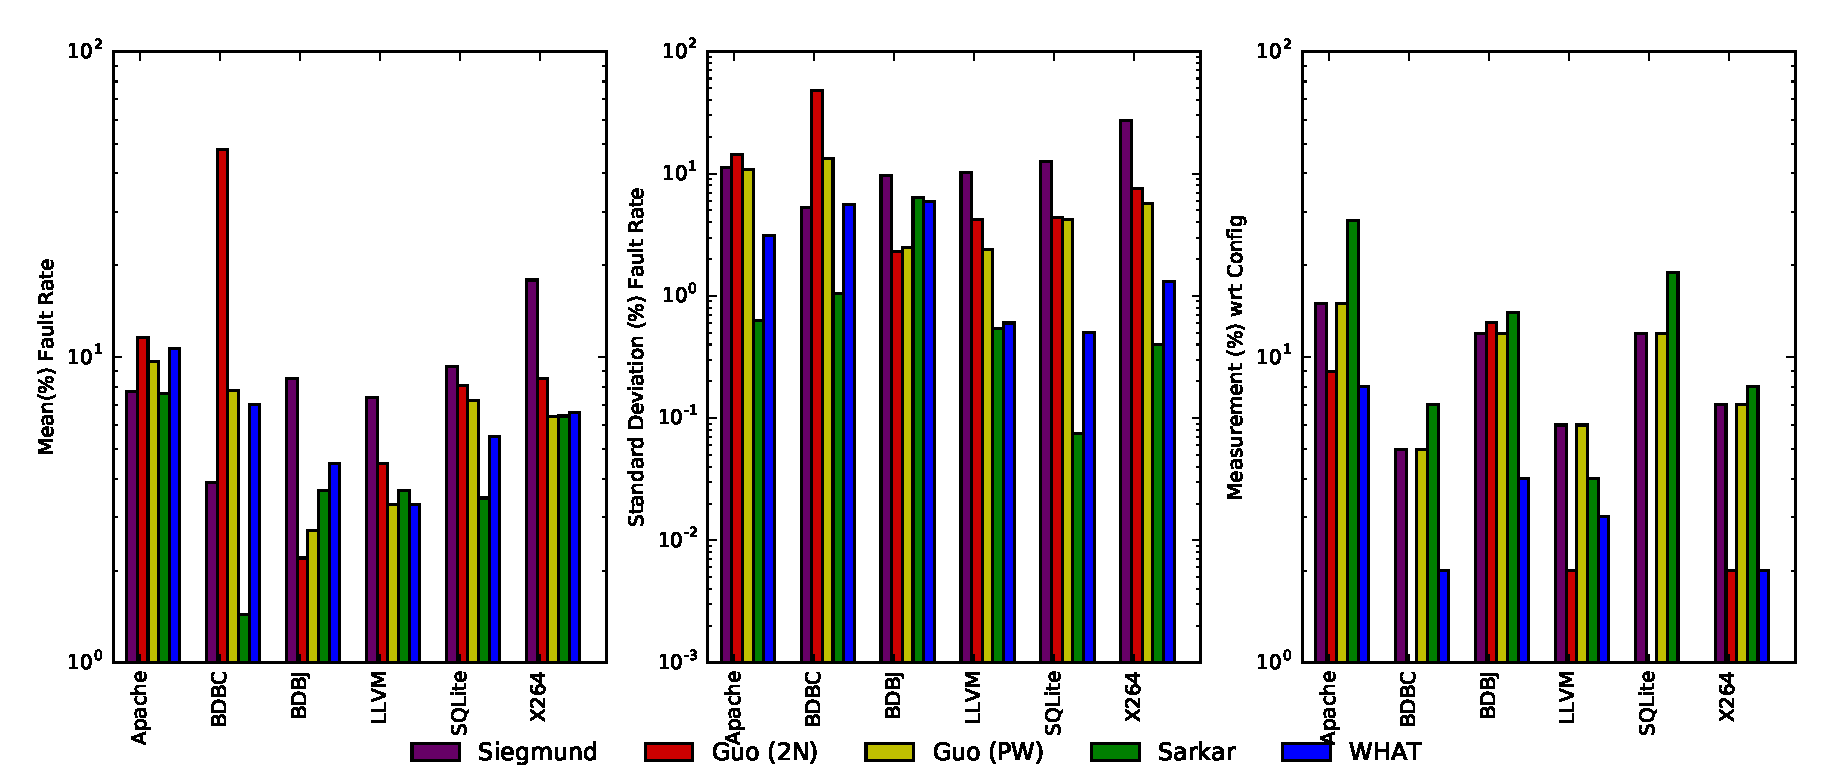
\includegraphics[width=\linewidth]{Figures/compare_graph_h.eps}
\caption{Comparison between various approaches proposed in the literature ~\cite{siegmund2012predicting}, \cite{guo2013variability}, \cite{sarkar2015cost}. The figure compares \what with other techniques w.r.t. the mean error, standard deviation, and the percentage configurations used for training the model.}\label{fig:Comparison}
\end{figure*}
 
{\em Compared to the start of the art in minimal sampling for
learning runtime predictors from product lines, how good is \what with $S_1$?}\\

We compare \what with the three state of the art predictors proposed in the literature~\cite{siegmund2012predicting}, \cite{guo2013variability}, \cite{sarkar2015cost}. Siegmund et al. proposed a method called feature-wise sampling (FW) and 
 another three elaborations (PW, HO, HS) of their basic method. We use PW since relies on relatively few data to build fairly accurate predictor. Guo et al. proposed progressive random sampling methodology, which samples in steps of the number of features in the software system. The termination criteria of this technique is based on the heuristic called as $PW$ similar to the one described in  Siegmund et al.. Sarkar et al. generates a small set of configurations, with help of a heuristic called feature-frequency,  to estimate the accuracy-measure curve. The estimation is done by comparing the points to a set of predefined basis functions. This estimated curve is then used to decide the optimal number of samples to achieve a threshold error rate.  
 
 In figure \ref{fig:Comparison}, we see that PW sampling of Siegmund et al. has the largest mean error rate in case of X264, where as Guo (2N) has the largest standard deviation in BDBC.  What is to be noticed here is \what can find a small number of solutions (under 10\,\%) that can then be used to build accurate predictors with very little variance (except in couple of cases). Figure \ref{fig:measurements} is presented to assert the fact that using \what, we are able to build accurate predictors by making few measurements.
 %Note that:
%  \bi
%     \item
    
%  \ei




% Please add the following required packages to your document preamble:
% \usepackage[table,xcdraw]{xcolor}
% If you use beamer only pass "xcolor=table" option, i.e. \documentclass[xcolor=table]{beamer}
\begin{table}[t]
\caption{Comparison of the number of the samples
required with the state of the art. The grey colored cells indicate the approach which has the lowest number of samples.  We notice that WHAT and Guo (2N) uses less data compared to other approaches. The high fault rate  of Guo (2N) accompanied with high variability in the predictions makes WHAT our preferred method.}\label{tab:measurements}
\vspace{2ex}
\centering
\small
\begin{tabular}{lrrrrr}
\toprule
                                   & \multicolumn{5}{c}{\textbf{Samples}}                                                                         \\ \cmidrule{2-6} 
\multirow{-2}{*}{\textbf{Dataset}} & \textbf{Siegmund} & \textbf{Guo (2N)}          & \textbf{Guo (PW)} & \textbf{Sarkar} & \textbf{\what}                \\ \midrule
\textbf{Apache}                    & 29                & 181                        & 29                & 55              & \cellcolor[HTML]{C0C0C0}16 \\ 
\textbf{BDBC}                      & 139               & \cellcolor[HTML]{C0C0C0}36 & 139               & 191             & 64                         \\ 
\textbf{BDBJ}                      & 48                & 52                         & 48                & 57              & \cellcolor[HTML]{C0C0C0}16 \\ 
\textbf{LLVM}                      & 62                & \cellcolor[HTML]{C0C0C0}22 & 64                & 43              & 32                         \\ 
\textbf{SQLite}                    & 566               & 78                         & 566               & 925             & \cellcolor[HTML]{C0C0C0}64 \\ 
\textbf{X264}                      & 81                & \cellcolor[HTML]{C0C0C0}32 & 81                & 93              & \cellcolor[HTML]{C0C0C0}32 \\ \bottomrule
\end{tabular}
\end{table}

% % Please add the following required packages to your document preamble:
% \usepackage{multirow}
% \usepackage[table,xcdraw]{xcolor}
% If you use beamer only pass "xcolor=table" option, i.e. \documentclass[xcolor=table]{beamer}
\begin{table*}[]
\centering
\caption{Comparison with Norbert et.al \cite{siegmund2012predicting}}
\label{my-label}
\begin{tabular}{|l|l|l|ll|l|l|}
\hline
                                   &                                              &                                            & \multicolumn{2}{l|}{\textbf{FaultRate(Them)}}                                    & \multicolumn{2}{l|}{\textbf{FaultRate(US)}}   \\ \cline{4-7} 
\multirow{-2}{*}{\textbf{Program}} & \multirow{-2}{*}{\textbf{Measurement(Them)}} & \multirow{-2}{*}{\textbf{Measurement(Us)}} & \multicolumn{1}{l|}{\textbf{Mean}}                & \textbf{Std}                 & \textbf{Mean}         & \textbf{Std}          \\ \hline
                                   & 15                                           &                                            & \multicolumn{1}{l|}{\cellcolor[HTML]{C0C0C0}44.1} & \cellcolor[HTML]{C0C0C0}42.3 &                       &                       \\ \cline{2-2} \cline{4-5}
                                   & 139                                          &                                            & \multicolumn{1}{l|}{3.9}                          & 5.3                          &                       &                       \\ \cline{2-2} \cline{4-5}
                                   & 160                                          &                                            & \multicolumn{1}{l|}{2.8}                          & 3.7                          &                       &                       \\ \cline{2-2} \cline{4-5}
\multirow{-4}{*}{BDBC}             & 164                                          & \multirow{-4}{*}{64}                       & \multicolumn{1}{l|}{2.8}                          & 3.7                          & \multirow{-4}{*}{9.3} & \multirow{-4}{*}{6.8} \\ \hline
                                   & 10                                           &                                            & \multicolumn{1}{l|}{\cellcolor[HTML]{C0C0C0}17.7} & \cellcolor[HTML]{C0C0C0}19.6 &                       &                       \\ \cline{2-2} \cline{4-5}
                                   & 48                                           &                                            & \multicolumn{1}{l|}{\cellcolor[HTML]{C0C0C0}8.5}  & \cellcolor[HTML]{C0C0C0}9.6  &                       &                       \\ \cline{2-2} \cline{4-5}
                                   & 116                                          &                                            & \multicolumn{1}{l|}{\cellcolor[HTML]{C0C0C0}3.8}  & \cellcolor[HTML]{C0C0C0}5.7  &                       &                       \\ \cline{2-2} \cline{4-5}
\multirow{-4}{*}{BDBJ}             & 162                                          & \multirow{-4}{*}{64}                       & \multicolumn{1}{l|}{1.7}                          & 3.5                          & \multirow{-4}{*}{2.7} & \multirow{-4}{*}{0.7} \\ \hline
                                   & 9                                            &                                            & \multicolumn{1}{l|}{\cellcolor[HTML]{C0C0C0}14.9} & \cellcolor[HTML]{C0C0C0}24.8 &                       &                       \\ \cline{2-2} \cline{4-5}
                                   & 29                                           &                                            & \multicolumn{1}{l|}{\cellcolor[HTML]{C0C0C0}7.7}  & \cellcolor[HTML]{C0C0C0}11.2 &                       &                       \\ \cline{2-2} \cline{4-5}
                                   & 80                                           &                                            & \multicolumn{1}{l|}{\cellcolor[HTML]{C0C0C0}11.6} & \cellcolor[HTML]{C0C0C0}22.7 &                       &                       \\ \cline{2-2} \cline{4-5}
\multirow{-4}{*}{Apache}           & 143                                          & \multirow{-4}{*}{16}                       & \multicolumn{1}{l|}{5.3}                          & 10.8                         & \multirow{-4}{*}{9.9} & \multirow{-4}{*}{2.4} \\ \hline
                                   & 26                                           &                                            & \multicolumn{1}{l|}{\cellcolor[HTML]{C0C0C0}7.8}  & \cellcolor[HTML]{C0C0C0}9.2  &                       &                       \\ \cline{2-2} \cline{4-5}
                                   & 566                                          &                                            & \multicolumn{1}{l|}{\cellcolor[HTML]{C0C0C0}9.3}  & \cellcolor[HTML]{C0C0C0}12.5 &                       &                       \\ \cline{2-2} \cline{4-5}
                                   & 566                                          &                                            & \multicolumn{1}{l|}{\cellcolor[HTML]{C0C0C0}7.1}  & \cellcolor[HTML]{C0C0C0}9.1  &                       &                       \\ \cline{2-2} \cline{4-5}
\multirow{-4}{*}{SQL}              & 569                                          & \multirow{-4}{*}{64}                       & \multicolumn{1}{l|}{\cellcolor[HTML]{C0C0C0}7}    & \cellcolor[HTML]{C0C0C0}9    & \multirow{-4}{*}{5.6} & \multirow{-4}{*}{0.2} \\ \hline
                                   & 11                                           &                                            & \multicolumn{1}{l|}{\cellcolor[HTML]{C0C0C0}7.8}  & \cellcolor[HTML]{C0C0C0}9    &                       &                       \\ \cline{2-2} \cline{4-5}
                                   & 62                                           &                                            & \multicolumn{1}{l|}{\cellcolor[HTML]{C0C0C0}7.4}  & \cellcolor[HTML]{C0C0C0}10.2 &                       &                       \\ \cline{2-2} \cline{4-5}
                                   & 62                                           &                                            & \multicolumn{1}{l|}{\cellcolor[HTML]{C0C0C0}7.4}  & \cellcolor[HTML]{C0C0C0}10.2 &                       &                       \\ \cline{2-2} \cline{4-5}
\multirow{-4}{*}{LLVM}             & 88                                           & \multirow{-4}{*}{32}                       & \multicolumn{1}{l|}{\cellcolor[HTML]{C0C0C0}5.7}  & \cellcolor[HTML]{C0C0C0}7    & \multirow{-4}{*}{3.3} & \multirow{-4}{*}{0.3} \\ \hline
                                   & 12                                           &                                            & \multicolumn{1}{l|}{\cellcolor[HTML]{C0C0C0}29.8} & \cellcolor[HTML]{C0C0C0}22   &                       &                       \\ \cline{2-2} \cline{4-5}
                                   & 81                                           &                                            & \multicolumn{1}{l|}{\cellcolor[HTML]{C0C0C0}17.9} & \cellcolor[HTML]{C0C0C0}27.2 &                       &                       \\ \cline{2-2} \cline{4-5}
                                   & 89                                           &                                            & \multicolumn{1}{l|}{5.1}                          & 15.1                         &                       &                       \\ \cline{2-2} \cline{4-5}
\multirow{-4}{*}{x264}             & 89                                           & \multirow{-4}{*}{32}                       & 5.1                                               & 15.1                         & \multirow{-4}{*}{6.6} & \multirow{-4}{*}{0.5} \\ \hline
\end{tabular}
\end{table*}

% % Please add the following required packages to your document preamble:
% \usepackage[table,xcdraw]{xcolor}
% If you use beamer only pass "xcolor=table" option, i.e. \documentclass[xcolor=table]{beamer}
\begin{figure*}[!t]
\centering
\begin{tabular}{|l|l|l|l|l|l|l|}
\hline
\thead{Dataset} & \thead{Mean Fault \\ Rate(Guo)} & \thead{Standard \\ Deviation(Guo)}   & \thead{Measurement \\ (Guo)} & \thead{Mean Fault \\ Rate(Us)} & \thead{Standard \\ Deviation(Us)} & \thead{Measurement \\ (Us)} \\ \hline
\textbf{Apache}  & \cellcolor[HTML]{C0C0C0}11.6  & \cellcolor[HTML]{C0C0C0}14.4  & \cellcolor[HTML]{C0C0C0}18 & 9.9                          & 2.4                         & 16                         \\ \hline
\textbf{LLVM}    & \cellcolor[HTML]{C0C0C0}4.5   & \cellcolor[HTML]{C0C0C0}4.2   & 22                         & 3.3                          & 0.3                         & 32                         \\ \hline
\textbf{X264}    & \cellcolor[HTML]{C0C0C0}8.5   & \cellcolor[HTML]{C0C0C0}7.5   & \cellcolor[HTML]{C0C0C0}32 & 6.6                          & 0.5                         & 32                         \\ \hline
\textbf{BDBC}    & \cellcolor[HTML]{C0C0C0}98.3  & \cellcolor[HTML]{C0C0C0}243.1 & 36                         & 9.3                          & 6.8                         & 64                         \\ \hline
\textbf{BDBJ}    & 2.2                           & \cellcolor[HTML]{C0C0C0}2.3   & 52                         & 2.7                          & 0.7                         & 64                         \\ \hline
\textbf{SQLite}  & \cellcolor[HTML]{C0C0C0}8.1   & \cellcolor[HTML]{C0C0C0}4.4   & \cellcolor[HTML]{C0C0C0}78 & 5.6                          & 0.2                         & 64                         \\ \hline
\end{tabular}
\caption{Comparison of
Guo et.al \cite{guo2013variability}, which uses $2*N$ number of configurations with WHAT + $S_1$ 
(shown in right-hand columns). Here N refers to the number of features of the software system (please refer to \cite{guo2013variability} for more details).  Gray denotes the cases where our method results in lower median fault rate and is more stable i.e. lower standard deviation. We see that our method does better in 3 out of 6 datasets. }\label{fig:guo_2n}
\end{figure*}

% % Please add the following required packages to your document preamble:
% \usepackage[table,xcdraw]{xcolor}
% If you use beamer only pass "xcolor=table" option, i.e. \documentclass[xcolor=table]{beamer}
\begin{figure*}[!t]
\centering
\begin{tabular}{|l|l|l|l|l|l|l|}
\hline
\thead{Dataset} & \thead{Mean Fault \\ Rate(Guo)} & \thead{Standard \\ Deviation(Guo)}   & \thead{Measurement \\ (Guo)} & \thead{Mean Fault \\ Rate(Us)} & \thead{Standard \\ Deviation(Us)} & \thead{Measurement \\ (Us)} \\ \hline
\textbf{Apache}  & 9.7                           & \cellcolor[HTML]{C0C0C0}10.8 & \cellcolor[HTML]{C0C0C0}29  & 9.9                          & 2.4                         & 16                         \\ \hline
\textbf{LLVM}    & 3.3                           & \cellcolor[HTML]{C0C0C0}2.4  & \cellcolor[HTML]{C0C0C0}64  & 3.3                          & 0.3                         & 32                         \\ \hline
\textbf{X264}    & 6.4                           & \cellcolor[HTML]{C0C0C0}5.7  & \cellcolor[HTML]{C0C0C0}81  & 6.6                          & 0.5                         & 32                         \\ \hline
\textbf{BDBC}    & 7.8                           & \cellcolor[HTML]{C0C0C0}13.2 & \cellcolor[HTML]{C0C0C0}139 & 9.3                          & 6.8                         & 64                         \\ \hline
\textbf{BDBJ}    & 2.7                           & \cellcolor[HTML]{C0C0C0}2.5  & 48                          & 2.7                          & 0.7                         & 64                         \\ \hline
\textbf{SQLite}  & \cellcolor[HTML]{C0C0C0}7.2   & \cellcolor[HTML]{C0C0C0}4.2  & \cellcolor[HTML]{C0C0C0}566 & 5.6                          & 0.2                         & 64                         \\ \hline
\end{tabular}
\caption{Comparison of
Guo et.al \cite{guo2013variability} with WHAT+$S_1$ 
(shown in right-hand columns). Gray denotes the cases where our method results in lower median fault rate and is more stable i.e. lower standard deviation. We see that our method does better in SQLite and close to prior works results using far less evaluation (except for BDBC).}\label{fig:guo_pw}
\end{figure*}

% \begin{figure*}[!t]
\centering
\begin{tabular}{|l|l|l|l|l|l|l|}
\hline
                                   & \multicolumn{3}{l|}{\textbf{Their}}                                                                                                                                                                                                  & \multicolumn{3}{l|}{\textbf{Us}}                                                                                                                                                                                           \\ \cline{2-7} 
\multirow{-2}{*}{\textbf{Dataset}} & \textbf{\begin{tabular}[c]{@{}l@{}}Mean Fault\\ Rate(Sarkar)\end{tabular}} & \textbf{\begin{tabular}[c]{@{}l@{}}Standard\\ Deviation(Sarkar)\end{tabular}} & \textbf{\begin{tabular}[c]{@{}l@{}}Measurement\\ (Sarkar)\end{tabular}} & \textbf{\begin{tabular}[c]{@{}l@{}}Mean Fault\\ Rate (Us)\end{tabular}} & \textbf{\begin{tabular}[c]{@{}l@{}}Standard\\ Deviation (Us)\end{tabular}} & \textbf{\begin{tabular}[c]{@{}l@{}}Measurement\\ (Us)\end{tabular}} \\ \hline
Apache                             & 7.61                                                                       & 0.63                                                                          & \cellcolor[HTML]{FD6864}55                                              & 9.9                                                                     & 2.4                                                                        & 16                                                                  \\ \hline
BDBC                               & 1.44                                                                       & 1.04                                                                          & \cellcolor[HTML]{FD6864}191                                             & 9.3                                                                     & 6.8                                                                        & 64                                                                  \\ \hline
BDBJ                               & \cellcolor[HTML]{C0C0C0}3.66                                               & \cellcolor[HTML]{C0C0C0}6.34                                                  & 57                                                                      & 2.7                                                                     & 0.7                                                                        & 64                                                                  \\ \hline
LLVM                               & \cellcolor[HTML]{C0C0C0}3.67                                               & \cellcolor[HTML]{C0C0C0}0.55                                                  & \cellcolor[HTML]{FD6864}43                                              & 3.3                                                                     & 0.3                                                                        & 32                                                                  \\ \hline
SQLite                             & 3.46                                                                       & 0.08                                                                          & \cellcolor[HTML]{FD6864}925                                             & 5.6                                                                     & 0.2                                                                        & 64                                                                  \\ \hline
X264                               & 6.43                                                                       & \cellcolor[HTML]{C0C0C0}0.4                                                   & \cellcolor[HTML]{FD6864}93                                              & 6.6                                                                     & 0.5                                                                        & 32                                                                  \\ \hline
\end{tabular}
\caption{
Comparison of
Sarkar et.al's \cite{sarkar2015cost} recommended method (projective sampling)  with  \what +$S_1$ 
(shown in right-hand columns). Gray denotes the cases where our method results in lower median fault rate and is more stable i.e. lower standard deviation. We see that out method performs almost similar (LLVM and X264) and sometime better (BDBJ). The cases where we see that Sarkar et. al's method works better than \what, they use any where between 3 ( Apache, BDBC) to 14 (SQLite) times more points.
} \label{fig:sarkar}
\end{figure*}

% \fig{vs2012} compares the errors found by  \what+ $S_1$:Random with those found by the minimal sampling
% methods from Siegmund et al. Note that:
% \bi
% \item
% Simple feature-wise (FW) sampling uses fewer samples that 
% other methods, but its mean error and/or standard deviation can be largest. Hence, a simple addition
% of the known performance scores for individual features is less reliable that the other methods.
% \item
% As to the other minimal sampling methods  (PW,HO,HS)  \what+$S_1$:Random always had a   lower mean
% error rate and a much lower standard deviation on the error.  
% \item In terms of number of samples required to make those predictions, \what+$S_1$:Random needed
% much less detail that PW or HO or HS
% \ei


% Guo et al. proposed progressively random sampling methodology which samples in steps of the number of features in the software system. The termination criteria of this technique is based on the heuristic called as $PW$ same as the one described in  Siegmund et al.

% \fig{guo_2n} compares the errors found by  \what+ $S_1$:Random with those found by the minimal sampling
% methods when it used $2*N$ samples. The number of configurations evaluated is very close to the  number of configurations evaluated by our method.

% \fig{guo_pw} compares the errors found by  \what+ $S_1$:Random with those found by the progressive sampling method  after allowing it to run till completion.

% Note that: 
% \bi
% \item
% Comparing the numbers in \fig{guo_2n}, our method is better than Guo et al. sampling method in terms of higher accuracy and lower standard deviation (more stability). When comparing numbers in the \fig{guo_pw} our method is very close to the mean fault rate (except for BDBJ) but significantly better in terms of stability and number of measurements especially in case SQLite.
% \item
% The results are a clear indication that random sampling in itself is not a good policy where as exploiting the underlying dimension (uses spectral clustering) can generate more accurate and stable predictors
% \ei


\begin{myshadowbox}
Hence, we answer {\bf RQ4} with ``yes'',
since our minimal sampling method yields predictions that are similar or more accurate that prior
work and rely on fewer samples.
\end{myshadowbox}


 \section{Related Work}
\label{sect:related}
 
In 2000, Shi and Maik~\cite{shi00} claimed the term ``spectral clustering'' as a reference to their normalized cuts
image
segmentation algorithm that  partitions data through a spectral (eigenvalue) analysis of the  
Laplacian representation of the similarity graph between instances in the data.

In 2003, Kamvar et al.~\cite{kamvar2003spectral}  generalized that definition saying that ``spectral learners''
were any data-mining algorithm that first replaced the raw
dimensions with those inferred from the spectrum (eigenvalues) of the affinity (a.k.a. distance)
matrix of the data, optionally adjusted via some normalization technique).

Our clustering based on first principal component splits the data on a   approximation to an eigenvector, found at each recursive level
of the data (as described in \tion{spect}). 
Hence, this  method is a ``spectral clusterer'' in the general Kamvar-sense. 
Note that
for software engineering data, we have
not found that Kamvar's normalization matrices are needed.

Regarding sampling, there are a wide range of methods know as experimental designs or designs of experiments~\cite{pukelsheim2006optimal}. They usually rely on fractional factorial designs as in the combinatorial testing community~\cite{Kuhn:2013}. 

Furthermore, there is a recent approach that learns {\em performance-influence models} for configurable software systems~\cite{SGA+15}. While this approach can handle even numeric features, it has similar sampling techniques for the Boolean features as reported in their earlier work~\cite{siegmund2012predicting}. Since we already compared to that earlier work and do not consider also numeric features, we did not compare our work to performance-influence models.
% (but perhaps if we were text mining
%on very large dimensional data, we would add in that normalization). 
 


\section{Reliability and Validity}\label{sect:construct}

{\em Reliability} refers to the consistency of the results obtained
from the research.  For example,   how well independent researchers
could reproduce the study? To increase external
reliability, this paper has taken care to either  clearly define our
algorithms or use implementations from the public domain
(SciKitLearn)~\cite{scikit-learn}. Also, all the data used in this work is available
on-line in the PROMISE code repository and all our algorithms
are on-line at github.com/ai-se/where.

{\em Validity} refers to the extent to which a piece of research actually
investigates what the researcher purports to investigate~\cite{SSA15}.
{\em Internal validity} checks if the differences found in
the treatments can be ascribed to the treatments under study. 

One internal validity issue with our experiments is the choice
of {\em training and testing} data sets discussed in 
\fig{systems}. Recall that while all our learners used the same
{\em testing} data set, our untuned learners were only given
access to {\em training}.

Another internal validity issues is {\em instrumentation}. The very low $\mu$ and $\sigma$ error values
reported in this study are so small that it is reasonable to ask they are due to some instrumentation
quirk, rather than due to using a clever sample strategy:
\begin{compactitem}
\item
We note that our low $\mu$ values are consistent with prior work.  Sarkar et al.~\cite{sarkar2015cost} report their CART predictions
(learned using all configurations executed and the performance scores collected) had  errors of around 4\,\% (calculated using \eq{err}). Recall from our introduction that the  $\mu$ error values  seen with the methods of this paper
can be slightly more than 4\,\%, which is to be expected since our predictive models were built using less
data. 
\item
As to our low $\sigma$ values, we note that when the  error values are so close to 0\,\%, the standard
deviation of the error is ``squeezed'' between zero and those errors. Hence, we would expect that
experimental rigs
that generate error values on the order of 5\,\% \eq{err} should have $\sigma$ values of $0\le \sigma \le 5$ (e.g. like those seen in our introduction).
\end{compactitem}

Regarding SQLite, we cannot measure all possible configurations in reasonable time. Hence, we sampled only 100 configurations to compare prediction and actual performance values. We are aware that this evaluation leaves room for outliers.
Also, we are aware that measurement bias can cause false interpretations~\cite{}. Since we aim at predicting performance for a special workload, we do not have to vary benchmarks.



{\em External validity}  We aimed at increasing the external validity by choosing programs from different domains with different configuration mechanisms and implemented with different programming languages. Furthermore, the programs used are deployed and used in the real world. Nevertheless, assuming the evaluations to be automatically transferable  to all configurable programs is not fair. To further strengthen the external validity, we run the model (generated by \textit{\what + $S_1$:Random} against other optimizers, such as NSGA-II and differential evolution algorithms\cite{storn1997differential}. This is to validate the fact that the model does not work only for GALE style of perturbation. In Table \ref{fig:external_validity}, we see that the models developed is valid for all searchers, as all searchers are able to find the near optimal solutions.




%That said, there exist some class of data mining papers for which
%tuning may not be required. Consider  Le Goues et al.'s 2012
%ICSE paper that used a evolutionary program to learn
%repairs to code~
%in that paper was ``can we fix any of the known bugs?''. Note
%that this criteria is a ``{\em competency}'' statement, and
%not a ``{\em better than}'' statement (the difference being that
%one is 
%``can do'' and the other is ``can do better''). For such
%competency claims, tuning is not necessary. However, as soon
%as {\em better than} enters the performance criteria then this
%becomes a race between competing methods. In such a race,
%it is unfair to hobble one competitor with poor tunings.



\section{Conclusions}

We have proposed to use a fast spectral clusterer (\what) along with three new sampling techniques which were tested on 6 real-world configurable software systems borrowed from the literature. The recommended method \textit{$S_1$:Random} achieves similar to lower fault rates while being stable, when compared our results to the state of the art methods. 
Except from the Berkeley DB system, our method performs more accurate than methods proposed by Siegmund et al.  ~\cite{siegmund2012predicting} and Guo et al. ~\cite{guo2013variability}. We achieve a similar accuracy and stability as the approach by Sarkar et al~\cite{sarkar2015cost}, while requiring far smaller number of configurations to be measured. We also show that the sampling method \textit{$S_1$:Random} can be used to make cheap (but stable) surrogates to the problems, which can be then used by various off the shelf optimizers to find the desired configuration. 
With the properties of  a fast clusterer along with minimal sampling technique, a simple surrogate builder, \what, should find increasing attention and application in the near future.



\vspace*{0.5mm}
 
 
\bibliographystyle{plain}

\balance
\bibliography{activeconfig}  
\end{document}

\section{Appendix}

\subsection{Evolutionary optimization algorithms} \label{ssec:appendix_1}
starts with an \textit{initial population} (randomly generated, based on some constraints). Since the solutions are drawn from a uniform distribution, typically, this diversity is desirable, although in some cases we might want to initialize all of the available parents to some best-known solution and proceed from there. The chosen \textit{evaluation function} must be capable of differentiating
between two individuals, i.e., it has to be able to rank one solution ahead
function, are favored to become parents for the next generation of offspring. 
A core function in evolutionary optimizers are the
\textit{reproduction} functions that generate   new solutions  probabilistically in the neighborhood of old solutions. This process continues till the a \"good enough\" solution is achieved or a hard limit on iterations are reached.  
    
    There has been extensive research in evolutionary algorithms in search-based software engineering.  For example, here is a list of search algorithms used widely in research: \textit{simulated annealing}\cite{bell2013limited, menzies2007business}; various genetic algorithms\cite{goldberg1979complexity} agumented by techniques such as
    (1)~smarter population subset selection~\cite{zit02,deb00afast};
    (2)~\textit{differential evolution} \cite{storn1997differential}
    (3)~\textit{tabu search and scatter search}\cite{nebro2008abyss, molina2007sspmo, glover1986general, beausoleil2006moss}; 
    (4)~\textit{particle swarm optimization}\cite{pan2008particle}; 
    (5)~numerous decomposition approaches that use heuristics to decompose the total space into small problems, then apply a response surface methods such
    as our own GALE\cite{krall2014gale,zuluaga2013active} algorithm.
    
    For this study, we applied three optimizers that are standards
    in the SE literature (NSGA-II~\cite{deb00afast} and SPEA2~\cite{zit02})
    as well as our own GALE algorithm~\cite{krall2014gale}).
    GALE uses the WHERE algorithm to find a direction of most useful
    mutation. Given leaf clusters, each with an {\em East,West} point
    then 
    GALE mutates the population of candidates in that leaf cluster towards
    which of {\em East,West} has better evaluation scores. These
    mutants become the data  that is cluster
    and mutated by WHERE in  generation $i+1$.
    
\subsection{Parameter Used}
We used the default parameters for NSGA-II and Differential Evolution (as recommended by the authors) where as the parameters used by GALE are as follows:
\begin{itemize}
\item $\mu$ = 100: population size;
\item $\omega$ = $\mu$: minimum size leaf clusters;
\item $\lambda$ = 3: premature stopping criteria (sets the maximum
allowed generations without any improvement
on any objective).
\item $\delta$ = 1: the ``accelerator'' that encourages larger
mutations;
\item $\gamma$ = 1.5: the ``brake'' that blocks excessive mutation.
\end{itemize}
\subsection{Parameter Bias} 
For this study, we did not do extensive parameter tuning:
NSGA-II and DE were run using their default
settings while GALE was run using the settings that
worked well on the first model we studied, which were
then frozen for the rest of this study. As documented
above, those parameters were:
\begin{itemize}
\item $\mu$ = 100: population size;
\item $\omega$ = $\mu$: minimum size leaf clusters;
\item $\lambda$ = 3: premature stopping criteria (sets the maximum
allowed generations without any improvement
on any objective).
\item $\delta$ = 1: the ``accelerator'' that encourages larger
mutations;
\item $\gamma$ = 1.5: the ``brake'' that blocks excessive mutation.
\end{itemize}

If this paper was arguing that these parameters were
somehow optimal, then it would be required to present
experiments defending the above settings. However, our
claim is less than that—we only aim to show that with
these settings, GALE does as well than standard searching
tools. In future work, we will explore other settings.




\end{document}